% vim: set spell : spelllang=en_gb
\documentclass{beamer}
\author{Chiel Kooijman\\ Supervisor: Diederik Roijers}
\title{Dynamic priority broadcasting channels:\\a multi-objective planning problem}
\usepackage{graphicx,amsmath}
\usepackage{verbatim}
\usepackage{subcaption}
\usetheme{boxes}
\usecolortheme[named=black]{structure}
\usepackage{xcolor}
%\usepackage[round]{natbib}
%\setbeamersize{text margin left=5pt,text margin right=5pt}

\begin{document}
\frame{\titlepage}

%\frame{\frametitle{Table of contents}\tableofcontents}


\begin{frame}{Dynamic priority broadcasting channels}
	Finding optimal policies for sharing a single resource (broadcasting
	channel) with multiple agents.
	\begin{figure}
		\centering
		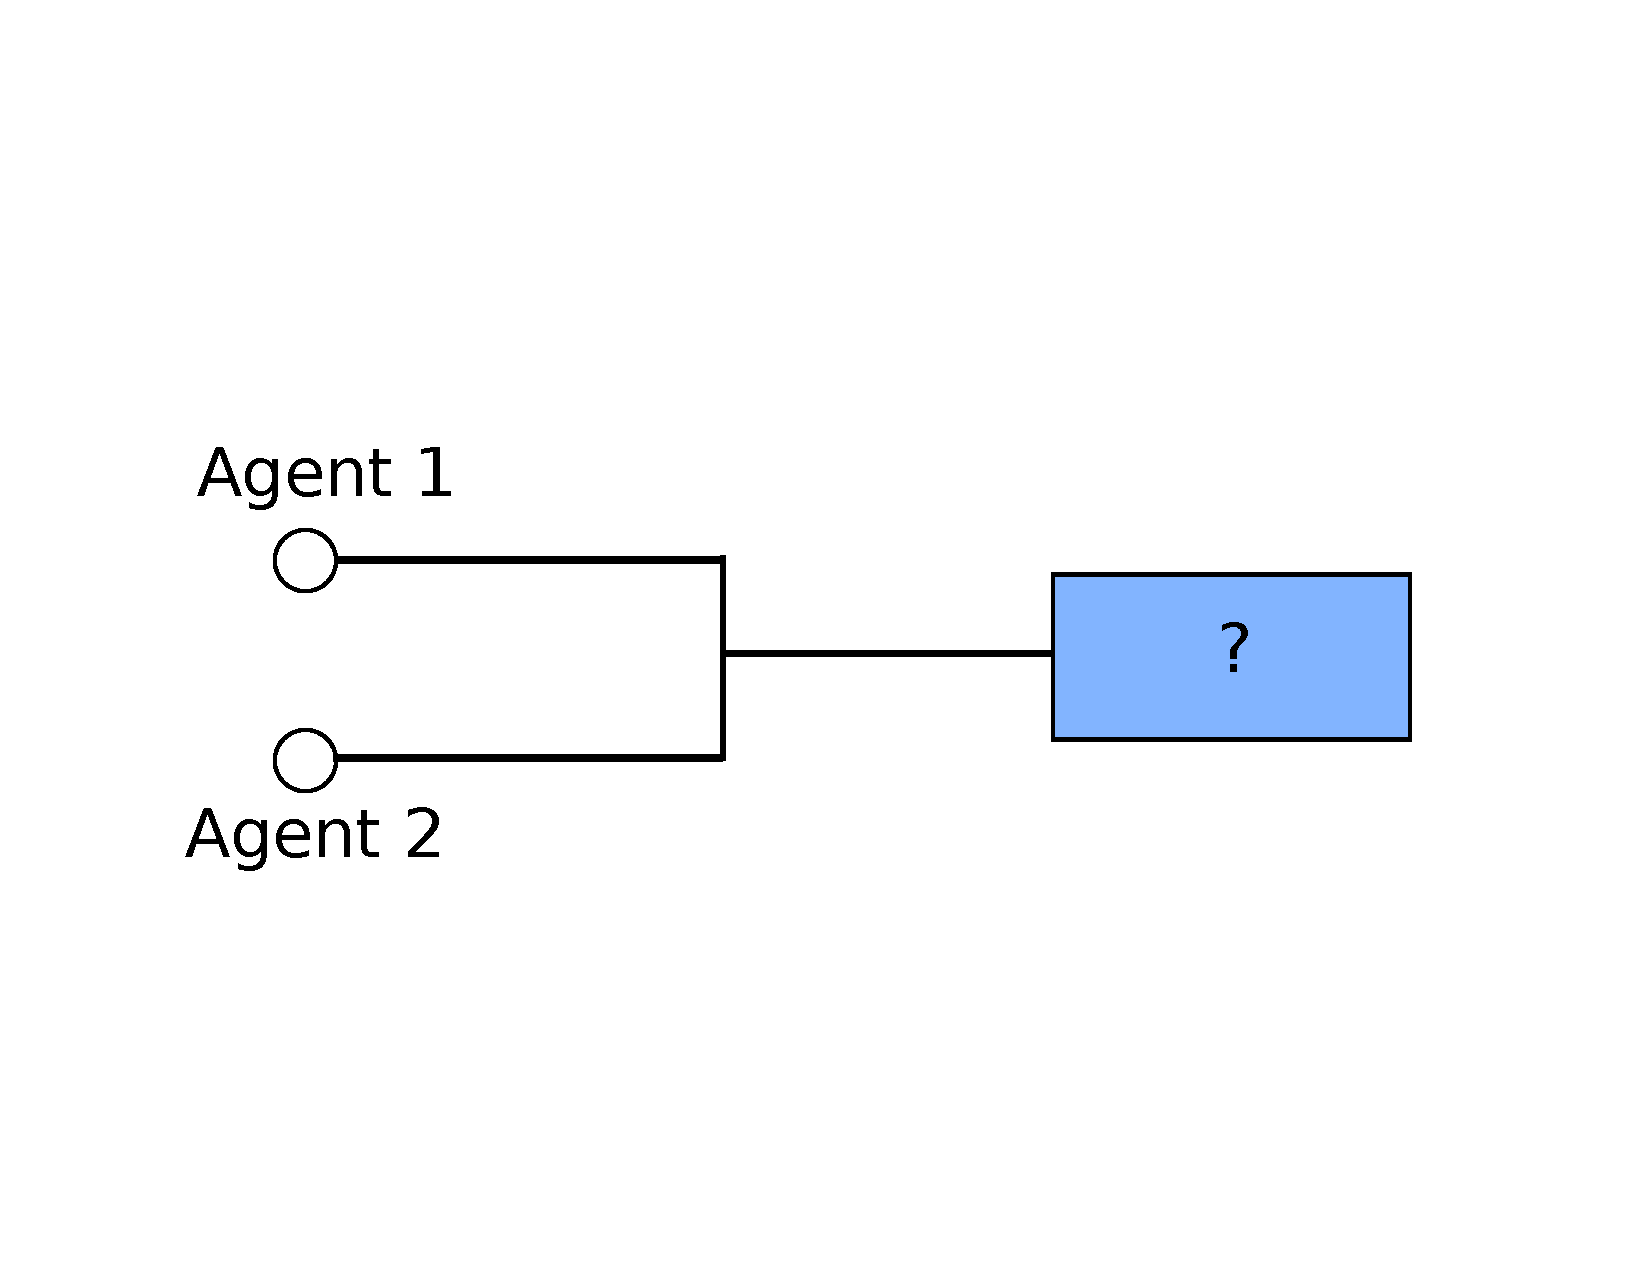
\includegraphics[scale=.3]{agents_ee}
	   \label{fig:agents_ee}
	\end{figure}
	\begin{itemize}
		\item The probability of an agent having a message to send is known.
		\item The reward for each agent sending a message is unknown in the
			planning stage.
	\end{itemize}
\end{frame}


\begin{frame}{Relevance}
	\begin{itemize}
		\item Several devices on a single connection (TV, telephone, PCs)
		\item For example:
		\begin{itemize}
			\item Emergency calls take priority
			\item Telephone calls always need a minimum of resources, but never
				the whole bandwidth
			\item Web browsing or gaming take priority over downloading large files
		\end{itemize}
	\end{itemize}
	\begin{figure}
		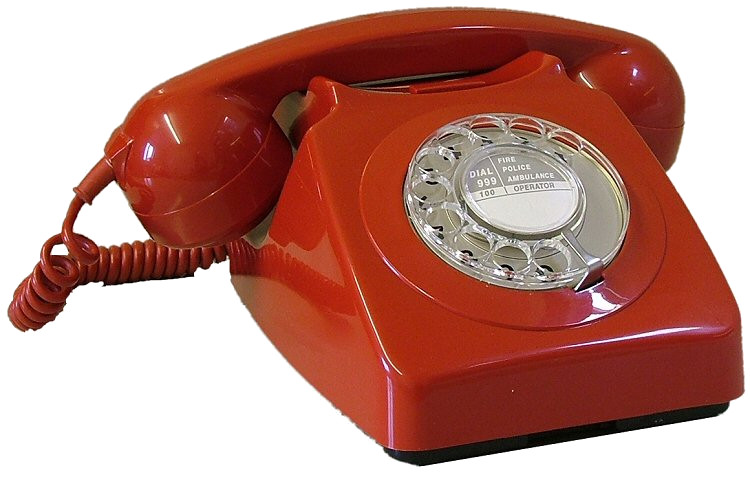
\includegraphics[height=5cm]{telephone}
	   \label{fig:telephone}
	\end{figure}
\end{frame}


\begin{frame}{Relevance}
	\begin{itemize}
		\item Prioritised load balancing in an operating system scheduler
		\begin{itemize}
			\item Increase responsiveness in consumer electronics
		\end{itemize}
		\item Efficiently sharing information over a single channel with multiple
			agents
	\end{itemize}
	\begin{figure}
		\caption{Agents sharing a single resource}
		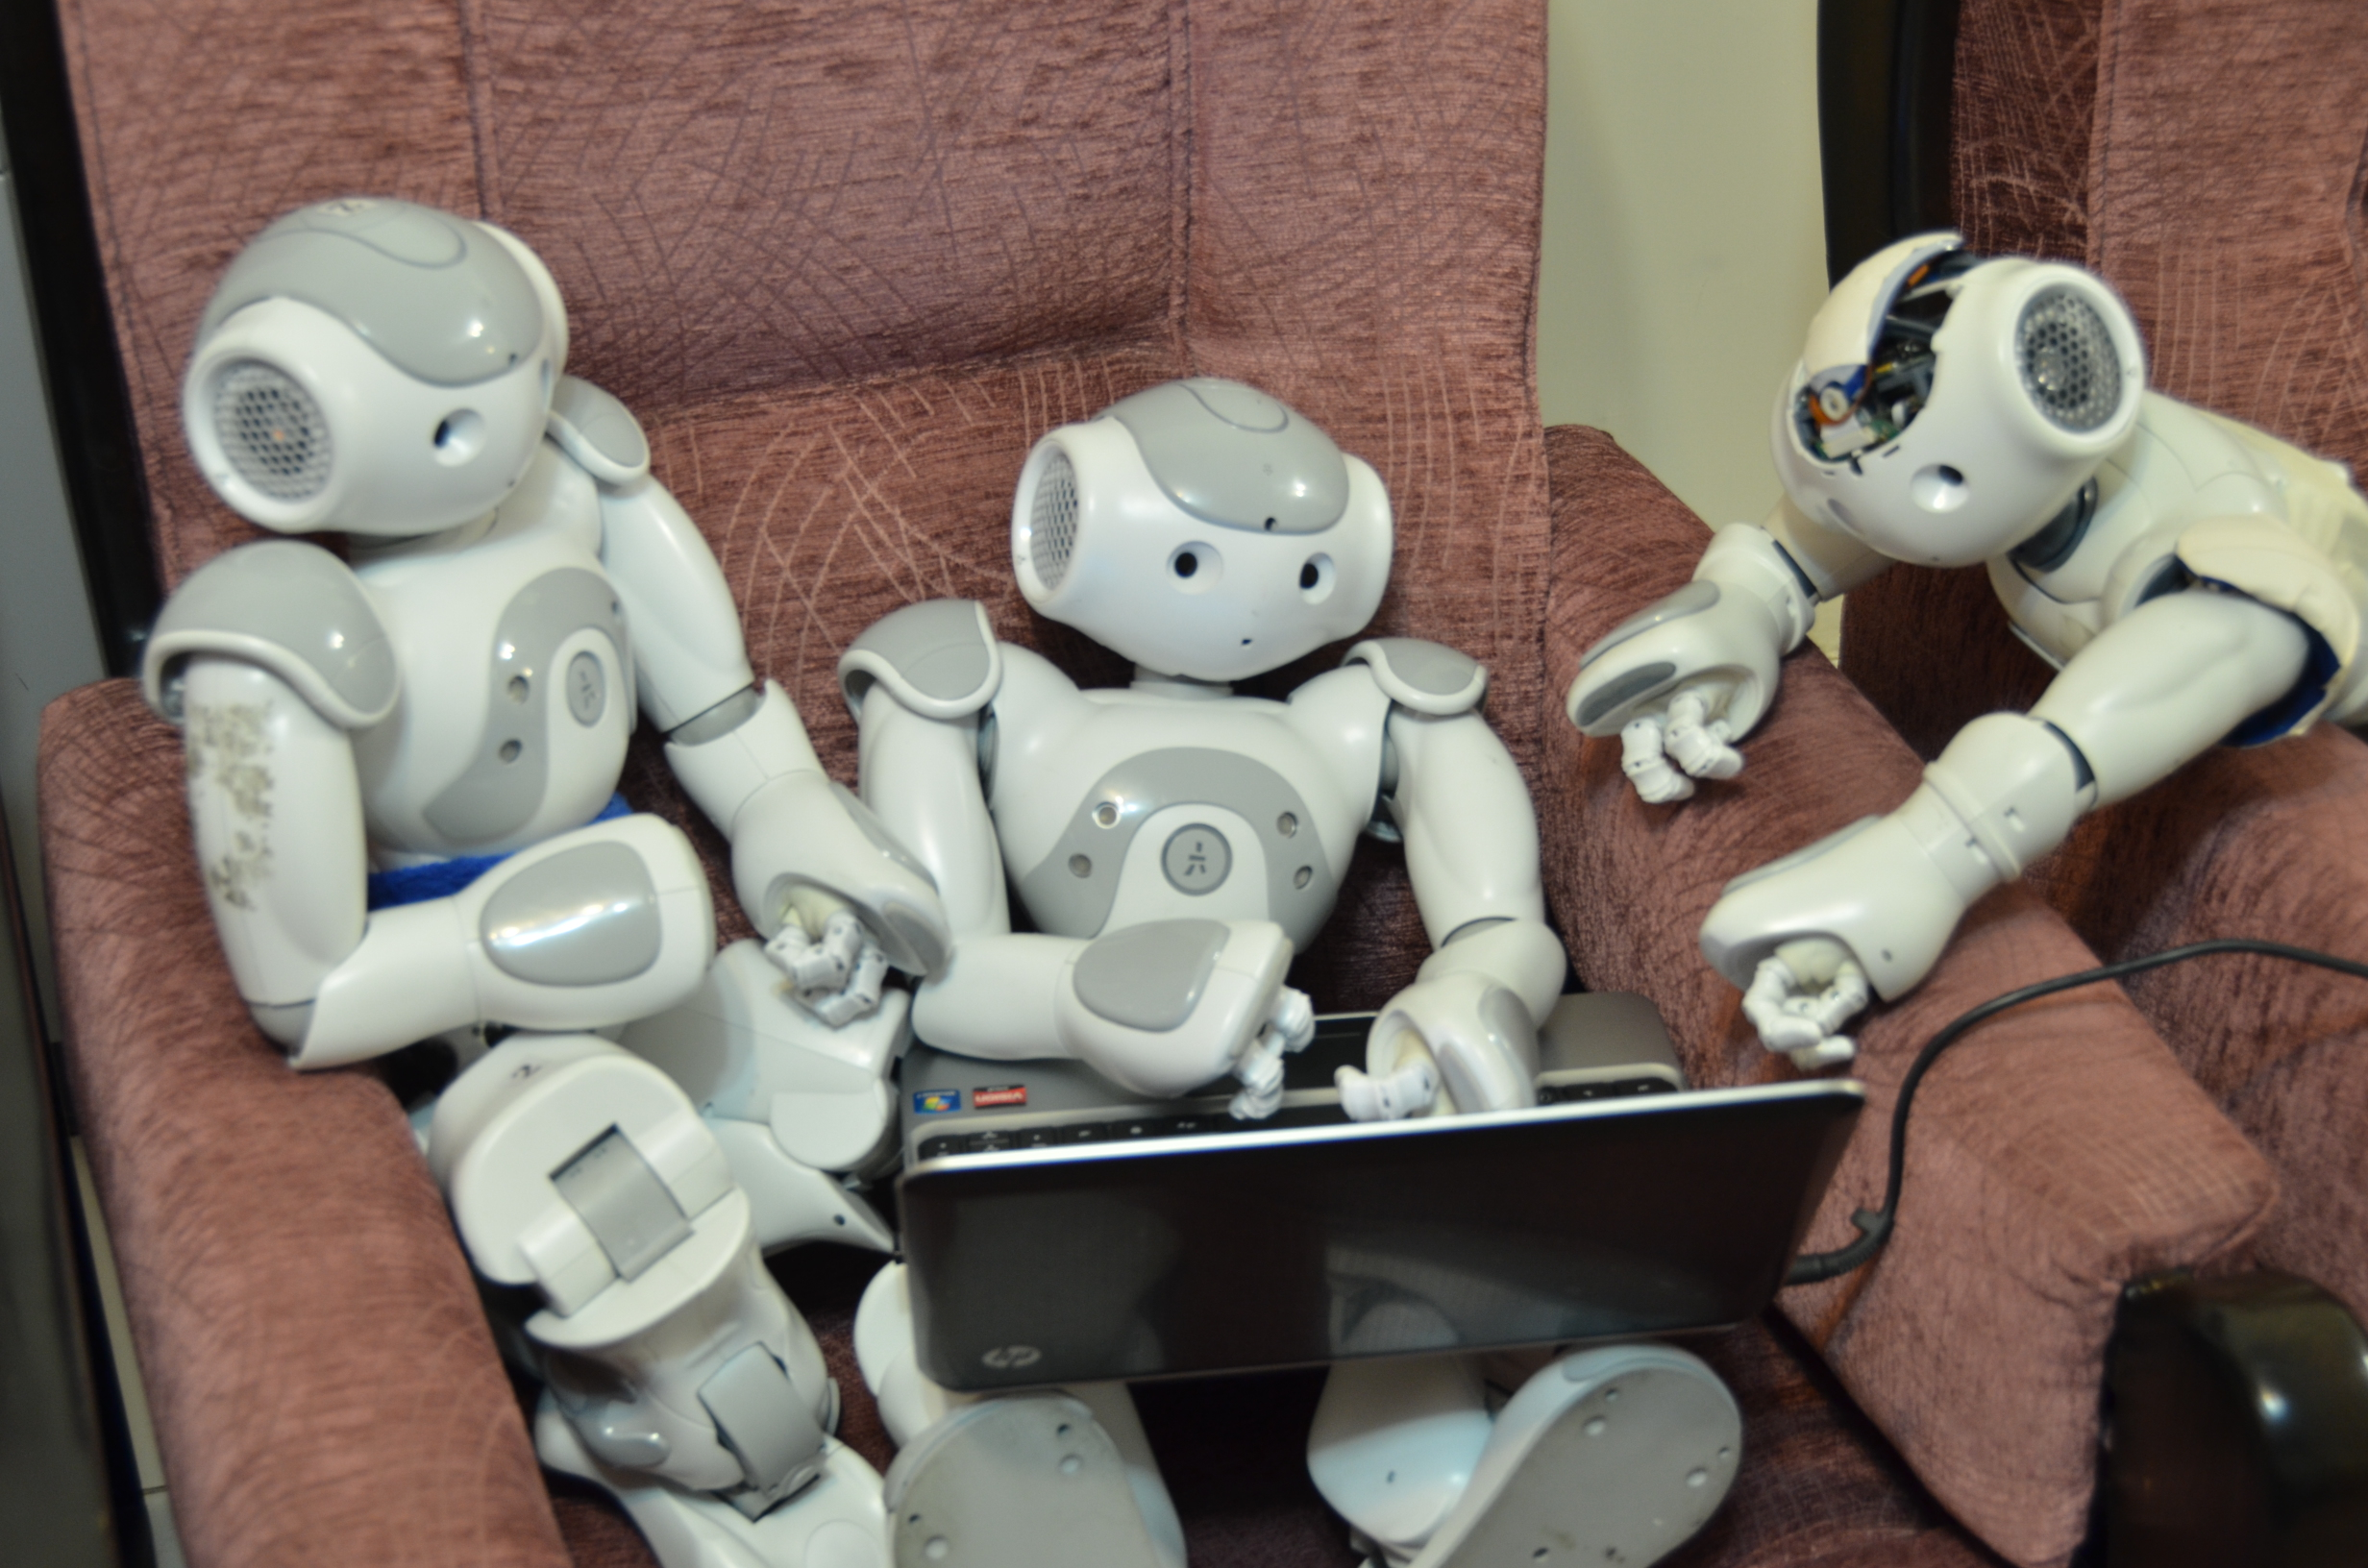
\includegraphics[height=5cm]{naos_pc}
	   \label{fig:naos_pc}
	\end{figure}
\end{frame}


\begin{frame}{Method}
	Calculate values for actions that represent expected return given that the
	optimal policy is followed.\\
	Bellman equation:
	$$ \displaystyle
	Q(s, a)^* = {\color{red}R(s, a)} + \sum_{s'} {\color{green}P(s'|s, a)}
	{\color{blue}\max_{a'} Q^*(s', a')}
	$$
	\begin{description}
		\item[{\color{red}$R(s, a)$}] Direct reward of action $a$
		\item[{\color{green}$P(s'|s, a)$}] Probability of ending up in $s'$ after doing $a$
		\item[{\color{blue}$\max_{a'} Q^*(s', a')$}] Value of the optimal action $a'$ in $s'$
	\end{description}
\end{frame}


\begin{frame}{Method}
	\begin{itemize}
		\item Number of states: $t \cdot 2^{n}$
		\item Number of possible actions (fully observable): $n+1$
		\item Number of possible actions (partially observable): $n!$
	\end{itemize}
	Easily extendible to multiple channels by changing reward for actions
	$$\begin{bmatrix}
		s\\
		\cdot\\
		s\\
		\cdot\\
	\end{bmatrix}
	\rightarrow
	\begin{bmatrix}
		0\\
		0\\
		0\\
		0\\
	\end{bmatrix}
	~\textrm{vs}~
	\begin{bmatrix}
		1\\
		0\\
		1\\
		0\\
	\end{bmatrix}$$
\end{frame}


\begin{frame}{Method}
	\begin{figure}
		\caption{Pareto-optimal set of solutions}
		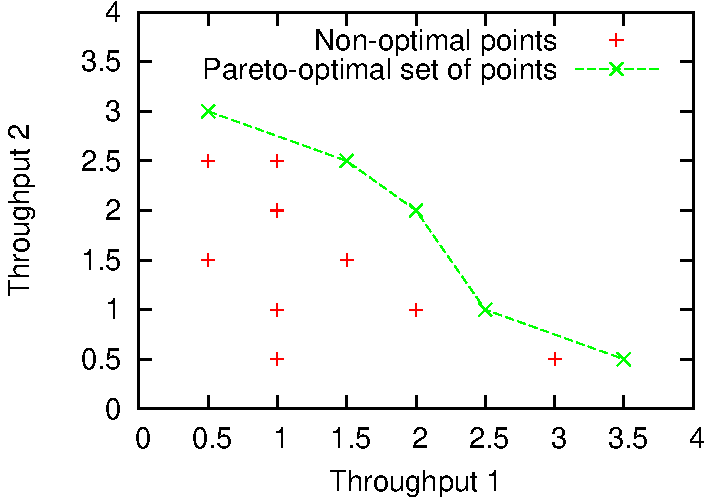
\includegraphics[scale=0.5]{../../images/pareto}
	   \label{fig:pareto}
	\end{figure}
	\begin{equation}
		\label{eq:pareto}
		\Big\{ V\, \Big| \, \forall V'[ V \neq V' \land \exists n [V_n > V'_n]] \Big\}
	\end{equation}
\end{frame}


\begin{frame}{Results}
	\begin{figure}
		\centering
		\begin{subfigure}[b]{0.3\textwidth}
			\centering
			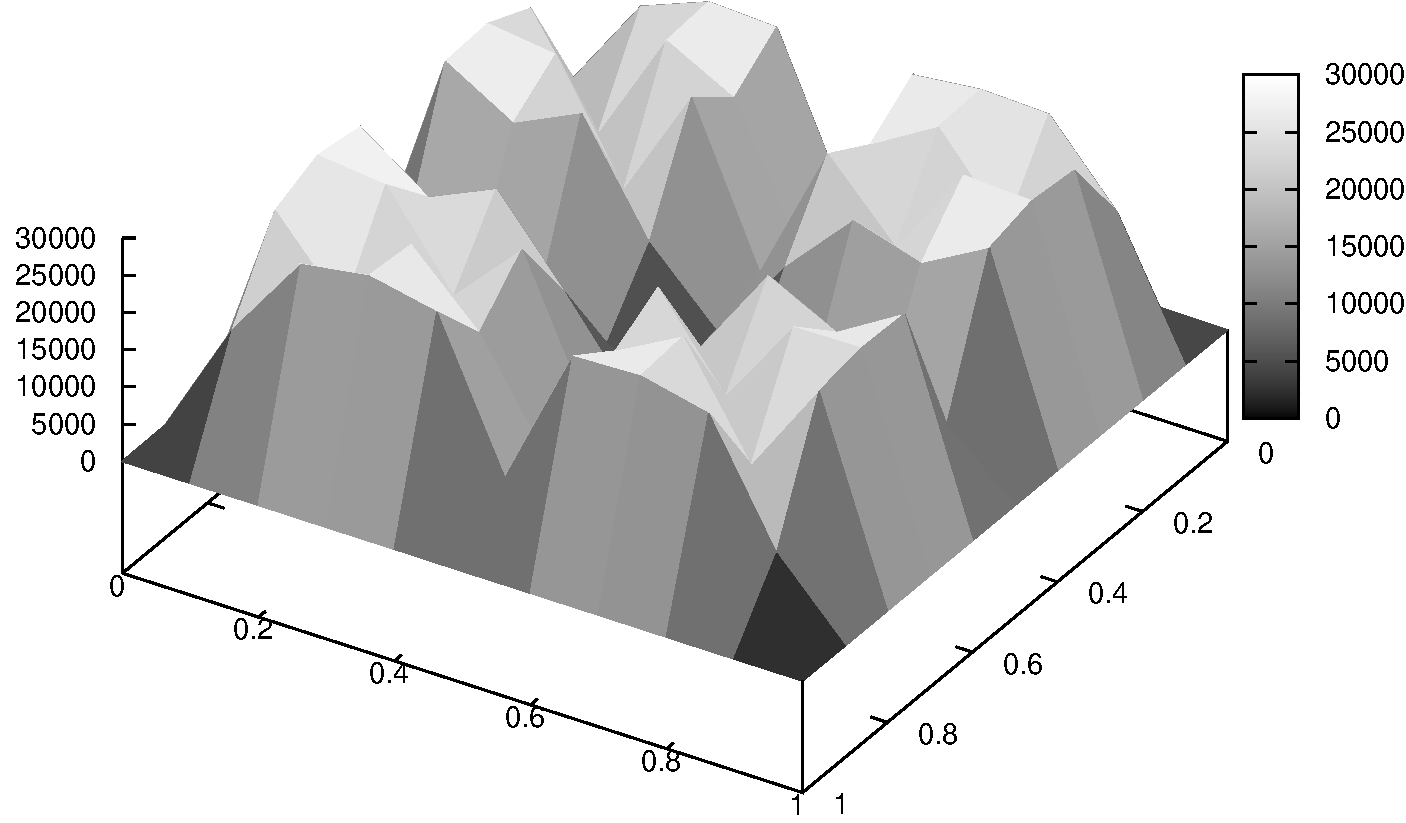
\includegraphics[height=2.8cm]{../../images/r3_nopareto}
			\caption{Without Pareto}
			\label{fig:../../images/r3_nopareto}
		\end{subfigure}
		\hspace{2cm}
		\begin{subfigure}[b]{0.3\textwidth}
			\centering
			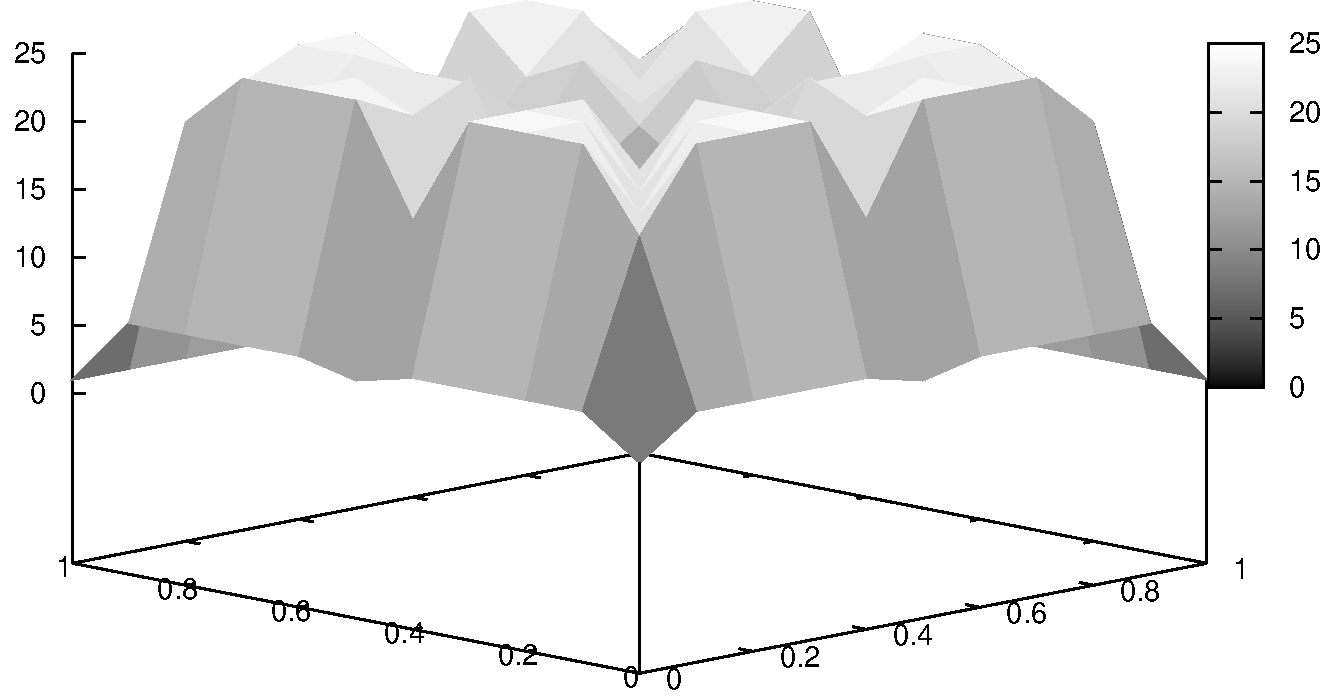
\includegraphics[height=2.2cm]{../../images/r3_diagonal}
			\caption{With Pareto}
			\label{fig:r3_diagonal}
		\end{subfigure}
		\caption{Reward set size at $t=3$}
	\end{figure}
	Set sizes differ only due to duplicate vectors All probability distributions
	benefit equally from Pareto optimisation (proportional to set size)
\end{frame}


\begin{frame}{Results}
	Pareto optimisation is faster (15 minutes to 4 seconds at $t=4$ for 2 agents)
	\begin{figure}
		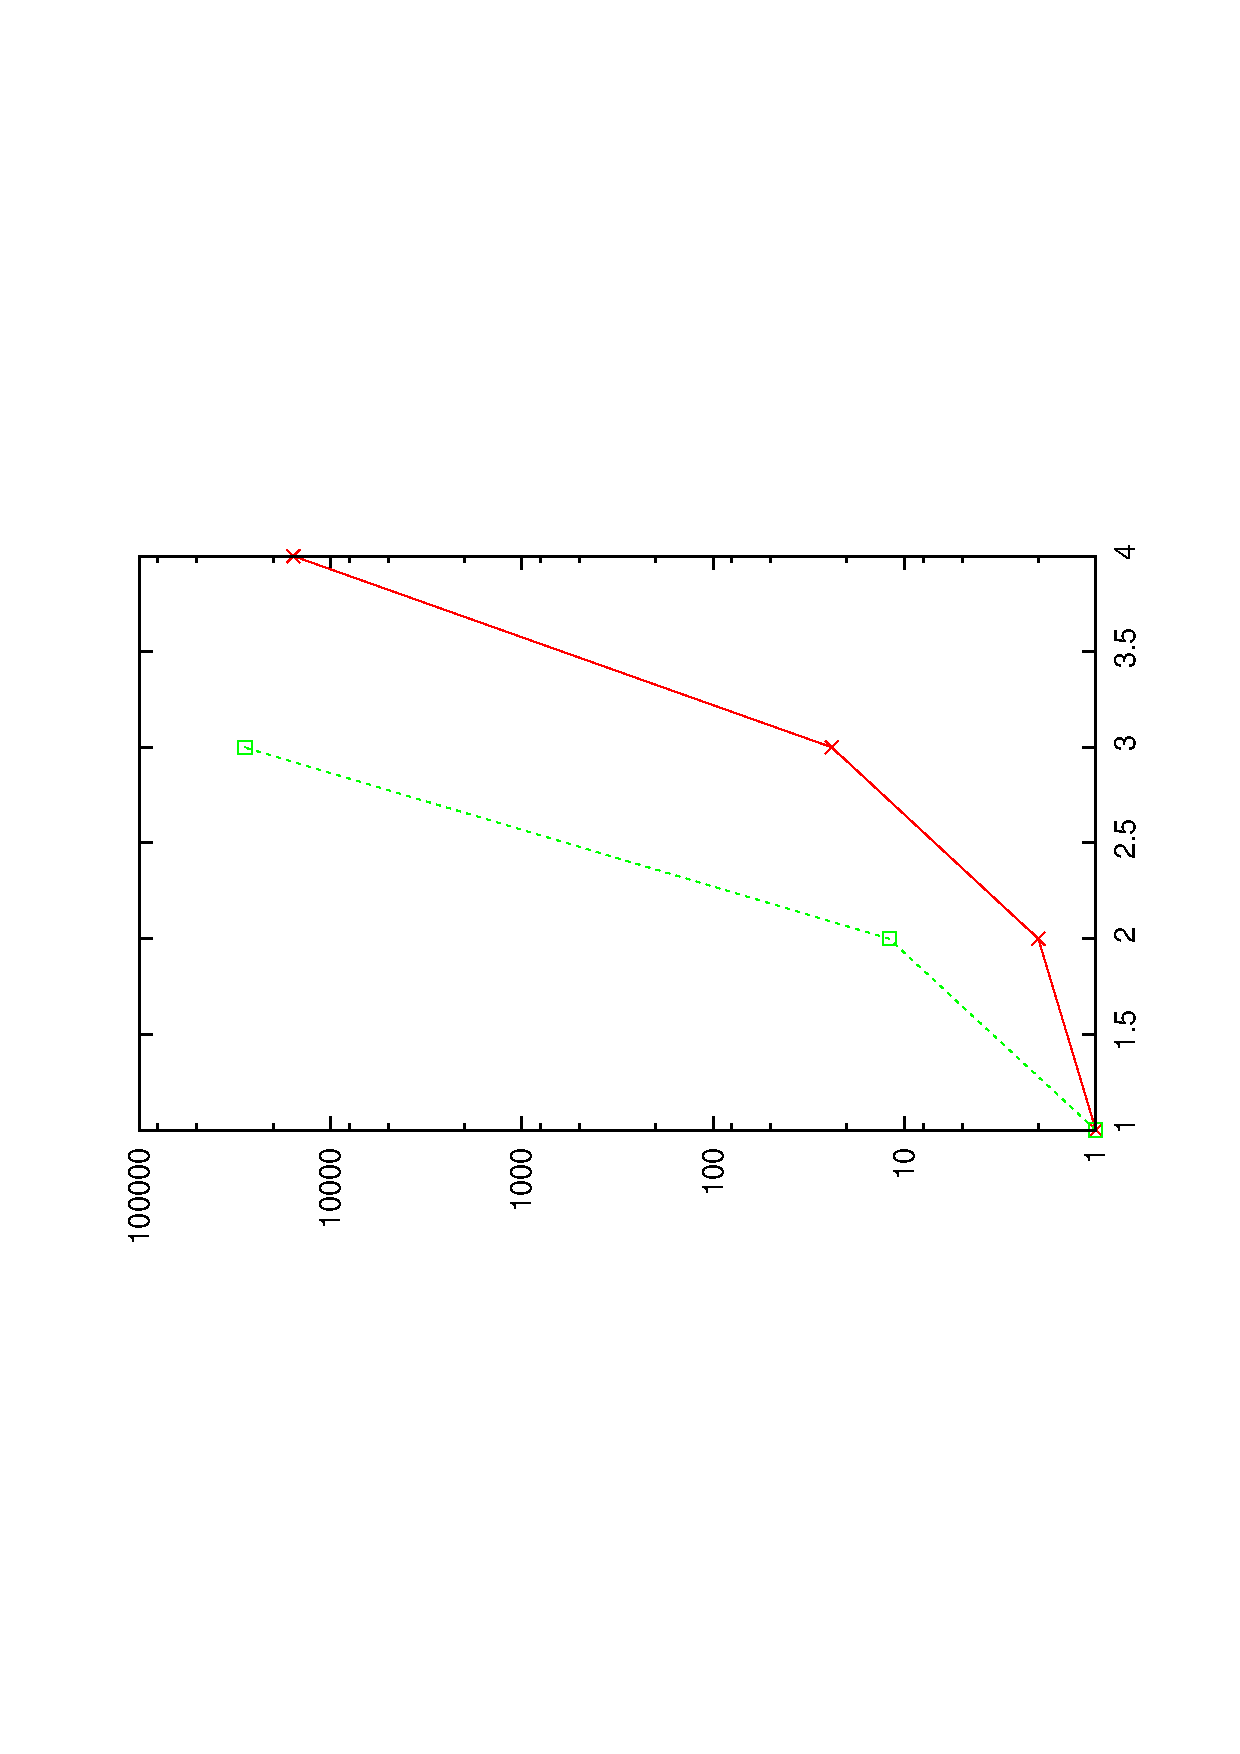
\includegraphics[scale=.3]{../../images/pareto_difference}
		\label{fig:../../images/pareto_difference}
		\caption{Size of Pareto-optimal set for number of time steps}
	\end{figure}
	Current implementation can not plan ahead more than 4 steps for 2 agents or
	2 for 3
\end{frame}


\begin{frame}[Results]
	$$ \displaystyle
	Q(s, a)^* = R(s, a) + {\color{red}\sum_{s'}} P(s'|s, a) {\color{red}\max_{a'}} Q^*(s', a')
	$$
\end{frame}


\begin{frame}{Future}
	Exploit sorted C++ set structure to compute the Pareto optimal set more
	efficiently:\\
	Insert $[2, 1, 2]$:\\
	\{\\
	$[0, 4, 1]$\\
	$[1, 3, 2]$\\
	$[2, 2, 3]$\\
	$[3, 1, 4]$\\
	$[4, 0, 5]$\\
	\}
\end{frame}


\begin{frame}{Future}
	Exploit sorted C++ set structure to compute the Pareto optimal set more
	efficiently:\\
	Insert $[2, 1, 2]$:\\
	\{\\
	$[{\color{red}0}, 4, 1]$\\
	$[{\color{red}1}, 3, 2]$\\
	$[2, 2, 3]$\\
	$[{\color{green}3}, 1, 4]$\\
	$[{\color{green}4}, 0, 5]$\\
	\}
\end{frame}


\begin{frame}{Future}
	Exploit sorted C++ set structure to compute the Pareto optimal set more
	efficiently:\\
	Insert $[2, 1, 2]$:\\
	\{\\
	$[{\color{red}0}, {\color{green}4}, 1]$ x\\
	$[{\color{red}1}, {\color{green}3}, 2]$ x\\
	$[2, {\color{green}2}, 3]$\\
	$[{\color{green}3}, 1, 4]$\\
	$[{\color{green}4}, {\color{red}0}, 5]$ x\\
	\}
\end{frame}


\begin{frame}{Future}
	Exploit sorted C++ set structure to compute the Pareto optimal set more
	efficiently:\\
	Insert {\color{red}$[2, 1, 2]$}:\\
	\{\\
	$[{\color{red}0}, {\color{green}4}, 1]$ x\\
	$[{\color{red}1}, {\color{green}3}, 2]$ x\\
	$[2, {\color{green}2}, {\color{green}3}]$\\
	$[{\color{green}3}, 1, {\color{green}4}]$\\
	$[{\color{green}4}, {\color{red}0}, 5]$ x\\
	\}
\end{frame}


\begin{frame}{Future}
	\begin{figure}
		\centering
		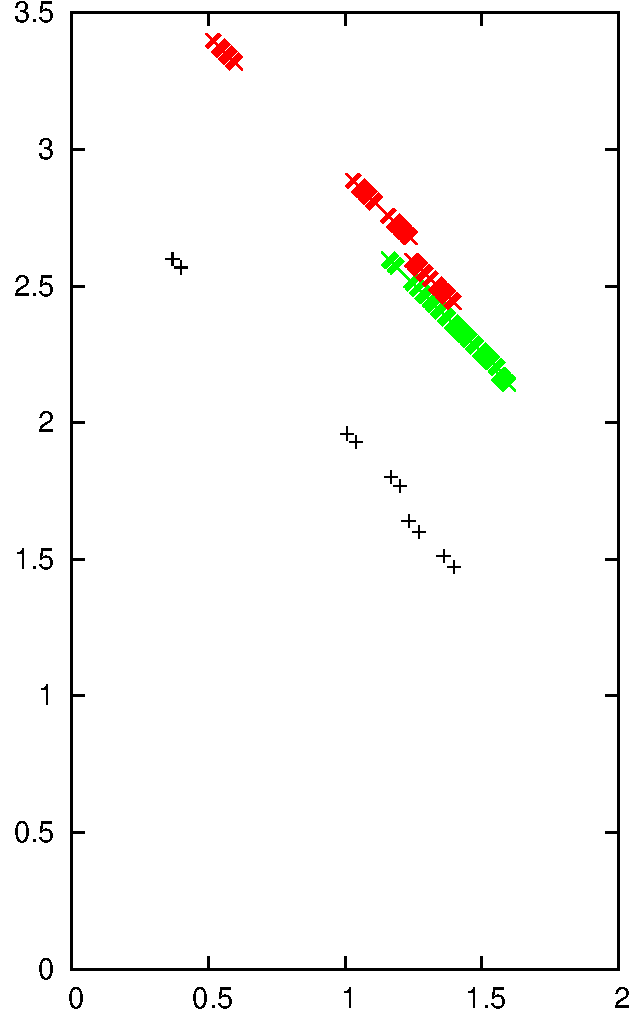
\includegraphics[height=5cm]{../../images/t4_28}
		\caption{Example of the Pareto sets with probabilities 0.2 and 0.8 ($t=4$)}
		\label{fig:t4_28}
	\end{figure}
	Pareto-optimal sets are divided in hyperplanes perpendicular to the origin
	(memory space)
\end{frame}

\begin{frame}{Conclusion}
	Memory requirements grow faster than exponential, so a more aggressive
	pruning method is needed.

	For example a minimum distance between vectors: $\varepsilon$-approximate
	pareto optimality \cite{barrett2008learning}.
\end{frame}

\begin{frame}
	\bibliographystyle{apalike}
	\bibliography{../../references}
\end{frame}
\end{document}
